\documentclass[conference]{IEEEtran}

\usepackage{hyperref}

\usepackage[utf8]{inputenc}
\usepackage{ifthen}
\usepackage{xcolor}
\usepackage{cite}
\usepackage[pdftex]{graphicx}
\graphicspath{{images/}}
\usepackage{tikz}
\usetikzlibrary{shapes,arrows,shadings,patterns}
\usepackage{pgfplots}
\pgfplotsset{compat=newest}
\pgfplotsset{plot coordinates/math parser=false}
\newlength\figureheight
\newlength\figurewidth

\usepackage{amsfonts}
\usepackage[cmex10]{amsmath}
\usepackage{multirow}

%\usepackage[hyphens]{url}
\usepackage{hyperref}
\def\UrlBreaks{\do\/\do-}

% Examples of several macros
%\newcommand*{\SET}[1]{\ensuremath{\boldsymbol{#1}}}
%\newcommand*{\VEC}[1]{\ensuremath{\boldsymbol{\mathrm{#1}}}}
%\newcommand*{\FAM}[1]{\ensuremath{\mathrm{#1}}}
%\newcommand*{\MAT}[1]{\ensuremath{\boldsymbol{\mathrm{#1}}}}
%\newcommand*{\OP}[1]{\ensuremath{\mathrm{#1}}}
%\newcommand*{\NORM}[1]{\ensuremath{\left\|#1\right\|}}
%\newcommand*{\DPR}[2]{\ensuremath{\left \langle #1,#2 \right \rangle}}

%\newtheorem{theorem}{Theorem}

%\newcommand{\alert}[1]{\textcolor{red}{#1}}
%\usepackage[caption=false,font=footnotesize]{subfig}
%\usepackage{url}

\pagestyle{plain}
\pagenumbering{arabic}

% correct bad hyphenation here
\hyphenation{mo-dule net-works semi-conduc-tor provi-ding}


\begin{document}
\title{Distributed Ledger for Depreciative Space Tracking Data}

\author{\IEEEauthorblockN{
Christian Dahdah\IEEEauthorrefmark{1},
Coline van Leeuwen\IEEEauthorrefmark{1},
Ziad Kheil\IEEEauthorrefmark{1},
Jérôme Lacan\IEEEauthorrefmark{1}
Jonathan Detchart\IEEEauthorrefmark{1} and
Thibault Gateau \IEEEauthorrefmark{1} 
}
\IEEEauthorblockA{\IEEEauthorrefmark{1}Institut Supérieur de l'Aéronautique et de l'Espace (ISAE-SUPAERO), Université de Toulouse, 31055 Toulouse, FRANCE\\
Email: \{al-cheikh-christian.el-dahdah, coline.van-leeuwen, ziad.kheil\}@student.isae-supaero.fr}
\IEEEauthorblockA{Email: \{jerome.lacan, jonathan.detchart, thibault.gateau\}@isae-supaero.fr}
}

\maketitle
\thispagestyle{plain}


\begin{abstract}
Blockchain, the technology that gained a lot of popularity with the price burst of Bitcoin in 2016, could be applied to increase transparency and cooperability between space agencies. In this work we underpin the importance of blockchain in satellite and debris tracking systems like in TruSat, a ConsenSys Space project. This paper proposes an innovative mechanism using Smart Contracts to exchange private keys in a public blockchain of encrypted data characterized fast depreciating value. Finally, we will demonstrate our mechanism using Solidity, Web3 and Golden Layout for visual interaction.

Keywords: Space Tracking, Space Debris, Smart Contract, Depreciative data, Golden Layout, Web3, Solidity, Trusat, Ethereum, Public Ledger
\end{abstract}

\IEEEpeerreviewmaketitle

\section{Context}
Modern spacecraft, whether destined to stay in Earth's orbit or leave its sphere of influence, are exposed to man-made debris. These debris proved to be of great danger for space exploration namely with the first confirmed accidental collision of a French satellite named \href{https://en.wikipedia.org/wiki/Cerise_(satellite)}{\textit{Cerise}} with a debris from an Ariane rocket. The incident was reported by \href{https://nssdc.gsfc.nasa.gov/nmc/spacecraft/display.action?id=1995-033B}{\textit{NASA and UK space track network}} and justified to the French government the need to build its own debris tracking system. Nowadays high profile space agencies rely on their own tracking systems, and intercommunication about possible collision is scarce and even primitive. The incident that happened on September 2, 2019 sets a good example: SpaceX did not respond to an ESA collision risk warning between Starlink 44 and Aeolus satellites because a glitch in the system prevented that.
% TODO
% source
% because of a glitch in the system?
% Which glitch ?

With no real solution to remove space junk, humankind is facing a real problem with more and more satellites being put in orbit. 
Since each collision produces more debris, there is a high risk of cascading collisions resulting in a ring of space debris around Earth. This scenario is known as Kessler's syndrome \cite{Kessler} named after the NASA scientist Donald J.Kessler.
Paradoxically,
our eagerness to thrive and conquer space may also one day hinder us from travelling outside our atmosphere. According to a 2020 \href{https://www.esa.int/Safety_Security/Space_Debris/Space_debris_by_the_numbers}{\textit{ESA safety and security report}}, there are 900 000 objects greater than 1cm-10cm of which the Space Surveillance Network is only regularly tracking more than 21 000 objects larger than 5-10 cm \cite{NasaOrbitalDebris}.

\section{Problem statement}
There are currently 34000 objects in space bigger than 10cm and the numbers are only getting bigger as no junk removal is envisaged in the near future. One collision could increase the risk dramatically. Let alone the infamous collision between Iridium 33 and Cosmos 2251 produced around 2000 large catalogued objects and 8 million fragments smaller than 1cm. Many studies show that the collision with a 1cm debris in LEO could be the equivalent of a hand grenade explosion, and the need for better tracking capabilities can't be stressed upon enough \cite{SmallDebrisImpact}. If we were to add objects bigger than 2cm to the tracking list, as \href{https://www.leolabs.space/}{\textit{LeoLabs}} anticipates, this adds a whopping 300 000 objects to the tracking list.

Luckily space object tracking is an ever growing interest for a lot of private companies like \href{https://northstar-data.com}{\textit{Northstar Earth and Space}} \cite{SpaceNews} \cite{Axios} and \href{https://www.leolabs.space/}{\textit{LeoLabs}} \cite{DigitalTrends} \cite{Axios}, privatisation is imminent. This growing market can be justified by the fact that in the upcoming 10 years, companies plan to orbit 12 000 satellites whereas as of 1957 until now only 9 600 satellites were successfully put in orbit hence more junk production and more satellites to maintain than ever before in the near future. In an effort to mitigate this problem, a solution is proposed to increase space agencies interoperability and promote the birth of new actors. In the absence of a real-time international space debris database, the use of a blockchain could reply to many problems.

\section{Potential contribution}
The term ``Blockchain'', is generally mistaken for cryptocurrencies like Bitcoin but this is as wrong as saying that the internet is google. Known in the literature as ``Public Ledger'', the technology's purpose is to run a code and publish information with the consent of all of its participants while not deleting any of the previous information. These properties prove to be interesting in the space tracking community \cite{BlockchainSpaceObjectLocation}. Publishing the position and the velocity in a Two Line Element (TLE) \cite{TwoLineSystem} format (often used in the literature) of a debris in a Public Ledger would greatly promote transparency between entities. A debris' history could be tracked, and pinpointing responsibilities would be more effective. As a result, \href{www.trusat.org}{TruSat} \cite{TruSat}, an open source project being developed by ConsenSys Space, is one of the most serious solutions addressing the problem of space debris. The project aims to have an international public ledger for satellites and debris' location while being the most certain about the authenticity of the published data. In order to understand the paper's objective and contribution, it is important to elucidate TruSat's engine and objective. 

The main idea of the latter is to design a system that lets anyone submit and contribute to the space tracking problematic, whether it is an individual with a smartphone's camera or a big company with sophisticated sensors and telescopes. The special feature (fig \ref{fig:TruSat and paper}) being developed is an engine that would evaluate the accuracy of one's information based on other participants' observations and distribute reputation points accordingly. Some key points to retain are that the system only awards reputation points to the first members that submitted a satellite's location, and others would only serve as witnesses to the accuracy of that information. Discovering and reporting a new debris would be the best way to increase one's trustworthiness. These points would serve to place each contributor in a special rank that is a direct reflection of their tracking value and capabilities. Furthermore, the ranks serve to distinguish between spammers and serious contenders. A rank 4 can validate a rank 0's data but not vice versa and people from the same rank cannot validate each other's information to avoid scammers. Lastly, the engine has an important function of suggesting which satellite lacks observation recordings and rewards generously the first contributor to report a recent observation of it. This would engage individuals to track different areas in the sky, thus having a more complete map of space and increasing cooperability. 

While Trusat's mission seeks to build a trustworthy network of space tracking enthusiasts, it does not address directly the creation of incentives that would engage people to participate in such a project. Since the project would be launched on the Ethereum mainnet, information is publicly accessible and free to read, thus making devoted entities unable to sustain themselves in such a system.

\begin{figure}[htp]
\centering
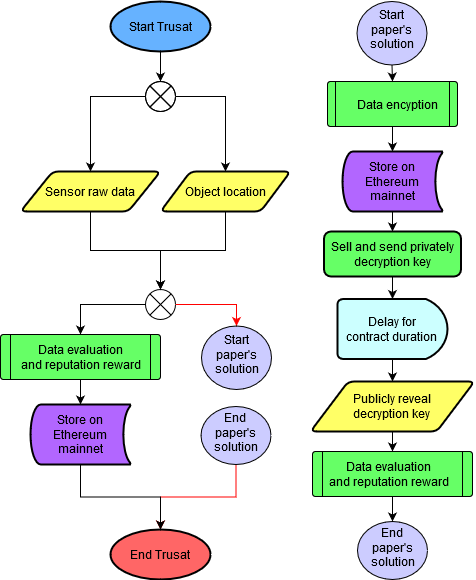
\includegraphics[width=\linewidth]{TruSat and paper.png}
 \caption{Flowchart depicting TruSat and the paper's proposed solution}
 \label{fig:TruSat and paper}
\end{figure}

To fill this gap, a solution suggested is to encrypt the data (fig \ref{fig:TruSat and paper}) off-blockchain and then to store it so that interested entities would have to buy the decryption key to read what was stored. However, to stay true to TruSat's objective it is fundamental to ensure that the encrypted data would be later revealed publicly so that:
\begin{enumerate}
  \item The provider would be evaluated for reputation and eliminate scammers.
  \item Co-operability and certainty of space object's location would be increased.
  \item Most importantly international transparency would be uplifted for satellites and debris tracking history.
\end{enumerate}
 
In this perspective, the paper introduces a new protocol that can be used safely on a public ledger to exchange information. The smart contract written works best for data which value has a fast depreciation rate like in the case of the aforementioned application.


\section{Protocol}
Before diving into the protocol that we put in place, some beforehand cryptography knowledge is necessary.

\medskip
\subsection{One Time Pad}
The One Time Pad (\textit{OTP}) \cite{OTP} (or Vernam cipher) is an encryption technique famously known for being \textit{the only completely unbreakable cipher}. It relies on generating a random, binary key as long as the message to encrypt, and producing the \textit{Exclusive-Or} (XOR, $\oplus$) of the two. 

\begin{figure}[htp]
  \centering
  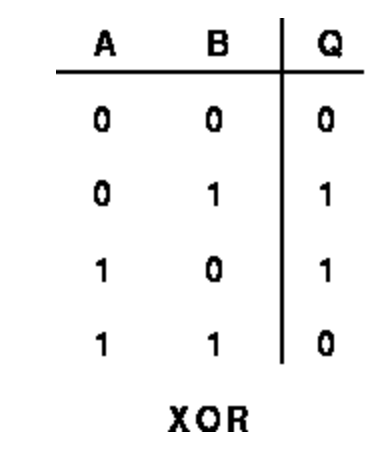
\includegraphics[width=3cm, height=3cm]{Xor.png}
  \caption{XOR truth table}
  \label{fig:truth-table}
\end{figure}

Although the length of the key has to be as long as the message, this encryption mechanism is completely unbreakable as long as the key is generated randomly and never used more than once.

To cut gas usage, we decided to apply a Stream Cipher method that closely resembles the OTP. However instead of working with a key the size of the message, a seed is used as the input of a pseudo-random generator which then returns the key needed to compute the XOR. This would not only drastically reduce the cost of storing a key on the blockchain, but also do so with a negligible loss in security.

\medskip
\subsection{Diffie-Hellman Key Exchange}

The Diffie-Hellman key exchange protocol is an asymmetric key algorithm designed to allow two users to securely share a secret key over an insecure public channel \cite{Diffie-Hellman}.
This secret key can then be used to securely exchange over the public channel, using symmetric key encryption algorithms.


Since its formulation in 1976 by Diffie and Hellman, the protocol has been widely used for securing online communications. 

The algorithm is based on multiplicative group of integers modulo n: ($\mathbb{Z}/n\mathbb{Z}$). If we take $n =p $ a prime number, in ($\mathbb{Z}/p\mathbb{Z}$ all $g \in [1,p-1]$ are primitive roots modulo p. This property results in the Diffie-Hellman Key Exchange protocol as follows:


If two users, Alice and Bob, want to safely exchange a secret key on a public channel with Eve as an eavesdropper:
\begin{itemize}
    \item They \textit{publicly} agree on a prime number \textbf{p} and a primitive root modulo p, \textbf{g}
    \item Alice chooses any secret integer \textbf{a}, and computes $\bf{A = g^a \mod{p}}$, then sends \textbf{A} over the public channel.
    \item Bob also chooses a secret integer \textbf{b}, computes $\bf{B = g^b \mod{p}}$, and sends \textbf{B}.
    \item Finally:
    \begin{itemize}
        \item Alice can compute the secret $S_1 = B^a \mod{p} $
        \item Bob can compute the secret $S_2 = A^b \mod{p} $
        \item Both Alice and Bob now share a common secret since $$S_1 = B^a \mod{p} $$
        $$= g^{ab} \mod{p} $$
        $$= A^b \mod{p}$$
        $$ = S_2 = \bf{S} $$
    \end{itemize}
\end{itemize}
If p is chosen as a very large prime (proven to be secure for lengths of $\sim$1000 digits and over), and a and b also are very large integers, Eve can not compute the secret given the public information.






\begin{table}[htp]
\centering
\large
\begin{tabular}{|c|c|c|}
\hline
\textbf{Alice} & \textbf{Bob} & \textbf{Eve} \\
\hline
  p,g & p,g & p,g  \\ 
 \textcolor{red}{a},A &  A &  A  \\ 
 B &  \textcolor{red}{b},B & B \\
 \hline
\end{tabular}
\large
\medskip
\caption{Visibility of Variables during the Diffie-Hellman Key protocol}
\label{my-label}
\end{table}

\subsection{The Protocol}


These two encryption schemes are used in our protocol to safely sell depreciative data to peers. Both the provider and the end user are guaranteed a scam proof transaction, validated by the smart contract to some extent (developed in section \ref{Future work section}).

The protocol (refer to fig. \ref{fig:Smart-Contract-Mechanism}, \ref{fig:Smart-Contract-Mechanism-2} and \ref{fig:Smart-Contract-Raise-Dispute} for clarity) can be explained in 10 key steps, and example use cases will be summarised in the next paragraph.
\begin{itemize}
    \item 1) Provider P wants to sell some information ``I'' deemed depreciative.
        \begin{itemize}
            \item Off blockchain, he generates a random key K of bytes long enough to encrypt ``I'' using the One Time Pad encryption (note that he can choose another encryption system if he wishes, as long as the client knows this).
            \item Off blockchain, he encrypts ``I'' with K, resulting in $$ I^{'} = K \oplus I $$
            \item Also off blockchain, P  generates two other keys: $(DH^{P}_{pr}, DH^{P}_{pu})$ which are the  Private and public keys of a Diffie-Hellman protocol.
            \item He deploys $I^{'}$ to the contract, with:
                \begin{itemize}
                    \item a certain price,
                    \item a description,
                    \item a number of days of validity N,
                    \item a minimum number of data he commits to provide,
                    \item  an amount in Ether representing an \textit{insurance fund} in the event he scams people (note that he can decide to put up no insurance funds, but this would probably be an odd behavior),
                    \item  his Diffie-Hellman public key $DH^{P}_{pu}$,
                    \item and an integer representing the price decrease because by essence the value of the information is lost over time. The decrease can be one of 3 options : 1 gives a linear decrease, 2 a quadratic decrease, and 0 or any other integer represents a constant price.
                \end{itemize}
            The contract assigns an identification number ``Id" to this information.

        \end{itemize}
    \item 2) A Client C decides to buy the information:
        \begin{itemize}
            \item C also generates two Diffie-Hellman keys (off blockchain): $(DH^{C}_{pr}, DH^{C}_{pu})$ which he stores.
            \item He calls the contract's buy function on Id, with the appropriate price and also provides his public key $DH^{C}_{pu}$. The ether he sends to the contract is stored in it and can be withdrawn by the client if step 3 is not accomplished.
        \end{itemize}
    \item 3) P sees that he has a new client, and needs to send him the key K.
    \begin{itemize}
        \item He generates (off blockchain) another random binary sequence $K_2$
        \item Off blockchain, P then combines his Diffie-Hellman keys $(DH^{P}_{pr}, DH^{P}_{pu})$ along with C's public key $DH^{C}_{pu}$ following the Diffie-Hellman algorithm, so C and P now have a shared secret key $K_3$.
        \item P then sends, through the D-app, $K \oplus K_2 \oplus K_3 $. Keep in mind that all miners and eavesdroppers can see this, but no one can decrypt it except for C.
    \end{itemize}
    \item 4) Now it is C's turn again :
    \begin{itemize}
        \item He gets $K \oplus K_2 \oplus K_3 $ by calling the contract.
        \item Just like P, he proceeds to combine his Diffie-Hellman keys $(DH^{C}_{pr}, DH^{C}_{pu})$ along with P's public key $DH^{P}_{pu}$ following the Diffie-Hellman algorithm, and now has $K_3$ as well.
        \item He can now simply compute: $K \oplus K_2 =  K \oplus K_2 \oplus K_3 \oplus K_3 $.
        \item Finally, C hashes the resulting binary $K \oplus K_2$ and sends it to the contract. (Note that the contract stores this hash).
    \end{itemize}
    \item 5) P reads the hash sent by C, and verifies that it is the correct hash because he can also compute it with the information he possesses. If it is wrong he stops the transaction, if not:
    \begin{itemize}
        \item He can now send $K_2$ , through the contract to the client C. The contract also stores $K_2$.
    \end{itemize}
    \item 6) Finally the client now has K2:
    \begin{itemize}
        \item He can compute $ K = K \oplus K_2 \oplus K_2$.
        \item Then, $ I = I^{'} \oplus K$.
    \end{itemize}
\end{itemize}

These 6 steps lead to a client having access to the message I, meanwhile eavesdroppers can not conclude anything. Note that another client also cannot circumnavigate the logic behind this, by using the same hash as the first client for example, because steps 2 to 5 need to be done for each client, thus the provider generates a different key $K_2$ for each client.

Finally, a few steps are left for the logic to be complete and to prevent fraud. Before the N days are over, the provider must:
\begin{itemize}
    \item 7) Reveal the key $K$, if he fails to do so he will not be able to withdraw his earnings and insurance funds, and clients will be refunded. Afterwards he must wait an additional 5 days.
\end{itemize}
During this time window, any client can set a \textit{dispute}. This means he deems that the key he was sold, does not correspond to K. 

\begin{itemize}
    \item 8) Clients who deem a fraud has happened must:
        \begin{itemize}
            \item Call the contract to raise a dispute using the identification Id of the product.
            \item The contract stores these funds and awaits for step 8.
        \end{itemize}
    \item 9) In the event of a dispute raised (fig. \ref{fig:Smart-Contract-Raise-Dispute}), the contract initiates the algorithm to settle the dispute:
    \begin{itemize}
        \item The D-app checks that a reference key $K$ was released by the provider, if not the client automatically wins the dispute.
        \item If the provider has not met the minimum data he promised, the client is also reimbursed. 
        \item If these two requirements are met, the contract must check if a fraud has happened on the reference key. The information the contract had stored was:
            \begin{itemize}
            \item the hash of $ K \oplus K_2 $ sent by the client and confirmed by the provider.
            \item The key $K_2$ sent by the provider.
            \item The key $K$ sent by the provider.
            \end{itemize}
        \item Thus, the contract can compute $ K \oplus K_2 $, and hash the result to confirm it really is what they agreed upon.

        \item Finally the contract allows the funds paid by the client, and the insurance deposit by the provider, to be retrieved by the party whom was right. This ensures that the correct person obtains the money.
    \end{itemize}
    \item 10) Finally after this 5 day window, the provider can withdraw his funds.
    \begin{itemize}
        \item He can withdraw the ether corresponding to the number of undisputed clients, clients who lost their disputes, and remaining funds from the insurance deposit.
        \item This operation can only be done once, and after the time frame has passed. No client can set a dispute after the provider withdraws his money.
 
    \end{itemize}
\end{itemize}

\begin{figure}[htp]
\centering
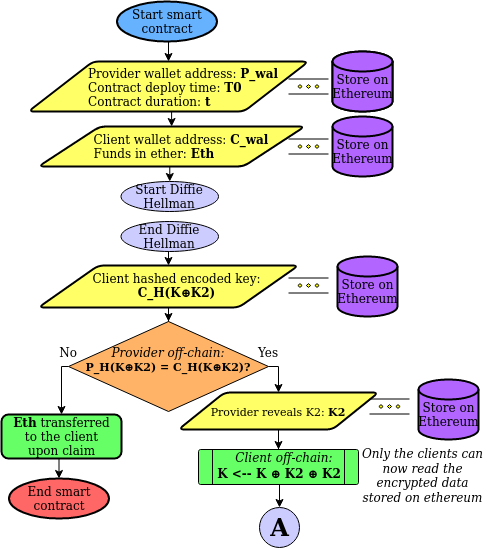
\includegraphics[width=\linewidth]{General mechanism.png}
 \caption{Flowchart depicting the smart contract's mechanism part1}
 \label{fig:Smart-Contract-Mechanism}
\end{figure}
 
\begin{figure}[htp]
\centering
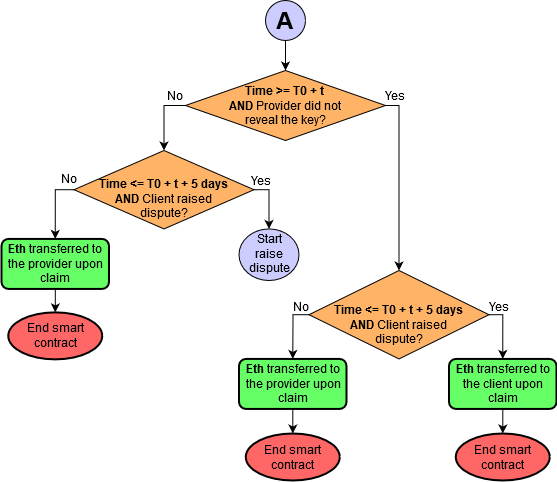
\includegraphics[width=\linewidth]{General mechanism 2.png}
 \caption{Flowchart depicting the smart contract's mechanism part2}
 \label{fig:Smart-Contract-Mechanism-2}
\end{figure}

\begin{figure}[htp]
\centering
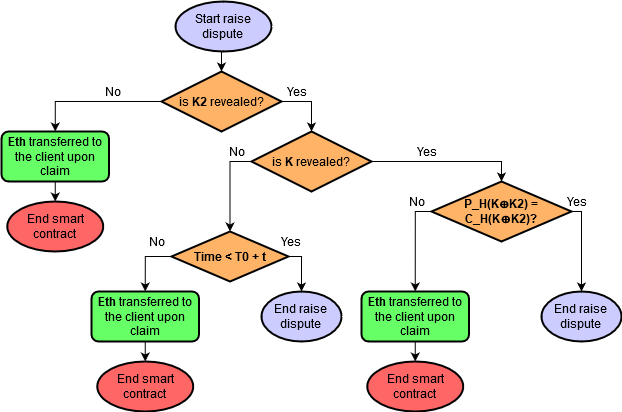
\includegraphics[width=\linewidth]{Raise dispute.png}
 \caption{Flowchart depicting the smart contract's raise dispute mechanism}
 \label{fig:Smart-Contract-Raise-Dispute}
\end{figure}


This protocol is derived from the desire to monitor frauds during transactions all the while maintaining the data sold encrypted on the ledger until it is deemed depreciated. The initial idea was for a client to simply send his public key, with which the provider would encrypt the reference key and send it back. The problem which arose was that no encryption contracts existed in solidity, thus the verification after a transaction was impossible. This protocol helped us bypass this issue because in reality, the client and provider both agree on the hash beforehand which is the real validation step. Furthermore computing a XOR and a hash is relatively simple in solidity.

\section{Implementation}

\subsection{Solidity}
Implementing the protocol was not straightforward as several factors had to be kept in mind before deploying the smart contract on Ethereum mainnet:
\begin{itemize}
    \item The gas price and gas limit.
    \item The block and transaction validation's time length had to be taken into account which is critical for fast depreciative data.
    \item The smart contract should be able to store any type of data for any application with just minor modifications.
\end{itemize}
\medskip
\subsubsection{Gas price and gas limit}
One of the main limitations that greatly impacts the contract's logic is the gas usage. The use of for-loops with an unknown number of iterations or searching in a table should be avoided in functions that do require gas. Consequently, in the proposed protocol when a provider \textbf{P} sets the encrypted data's key \textbf{K}, it is best not to compare automatically the hashes of $ K = K \oplus K_2$ with the one provided by each client to settle disputes because it requires a loop with a number of iterations that depends on the number of clients. Raising a dispute would require a special transaction from each client in order to claim the funds in the case of a fraud.

Moreover, selling a product requires the initialisation and storage of a lot of variables: deploy time, product end time, provider's address, initial price, depreciation type, insurance deposit, key \textbf{K}, clients addresses and their respective \textbf{$K_2$}, hashes and funds. This sets a significant gas price to sell multiple TLEs or any other product that needs to be updated often, which is to be impractical. For this matter it was best seen to group a set of TLEs (or products) into one reference that use the same encryption key \textbf{K}. This would be convenient for both the provider and the client. Grouping multiple sets of data implies exchanging less keys and calling less functions to buy/withdraw funds or raise a dispute.


In addition, many of the variables are destined to establish the communication protocol and securely transmit information between a provider and his clients. Storing these variables on the blockchain would be pointless because they don't directly intervene in the key verification process, which is the essence of the D-App. Thus, to cut gas costs, Events were often used in our design. This is the case for all Diffie-Hellman related keys, the transmission of $K \oplus K_2 \oplus K_3$ and the reference description. Since these variables play no role in the final verification process, the smart contract won't read them at any point thus we only emit them as events.

Note that the encrypted message could also have been emitted instead of stored to cut gas costs. However we deliberately chose to write this on the blockchain, since a reputation system is mandatory in parallel of the depreciation contract (later in section \ref{Future work section}). Storing the message can and will probably be vital for such a system.

\medskip

\subsubsection{Block validation time and transaction delay}
The process of creating a new reference of products, uploading data (TLEs in our case), buying them, and then exchanging keys can take several minutes or even hours on Ethereum, depending on the gas price and other factors set by each of the client and the provider. Therefore the contract cannot be functional for products that have a really fast depreciative rate, unless the client buys (or subscribes to) the reference beforehand, gets the keys and then the provider begins to upload the promised data. To clear things up, let us consider the following example: a client \textbf{C} has a satellite of altitude 800km and needs to have a mapping of debris at this orbit. A provider \textbf{P} sets a reference with a description stating that it will provide information the upcoming two weeks of debris in LEO of altitude 600 - 1000km with a minimum number \textbf{N} of TLEs. Client \textbf{C} subscribes to the reference and begins the key exchange protocol. After an hour, the client \textbf{C} is capable of reading the encrypted data that will be regularly uploaded by the provider \textbf{P} in the upcoming two weeks. In this setting the client will be able to access critical information in real time without any delay. At the end of the reference time, if the provider did not upload at least the minimum number \textbf{N} of TLEs promised, the client can raise a dispute and claim his funds.

Furthermore, getting the absolute time in a smart contract depends on the block it was mined in. This could raise security problems and multiple exploitation opportunities. For example a malicious node could mine a block and alter the time it mined it such as making a dispute could be in favor of a client instead of a provider. Knowing that an Ethereum block is mined on average every 14s-15s, relying on the number of blocks mined as a time reference could offset the contract duration by many days for a long term contract which is not practical. Fortunately block timestamps cannot be tempered a lot. A block with an abnormal timestamp \cite{Blockstamp} is rejected by the network. On the long run the timestamp could be offset by few minutes which is acceptable for this type of application.
\medskip
\subsubsection{Smart contract versatility and organisation} 
For clarity and ease of use, the protocol mechanism (excluding the TLE data type) was distributed over three solidity files:
\begin{itemize}
    \item {``Depreciation$\_$Contract.sol'' contains all the needed variables for the protocol inside the structure ``DataReference''. In addition the contract contains view functions that are common to both the client and the provider.}
    \item {``Client$\_$Depreciation$\_$Contract.sol'' inherits from ``Depreciation$\_$Contract.sol'', and implements all the functions needed on the client side such as buying a reference, raising a dispute, and setting the hash.}
    \item {``Provider$\_$Depreciation$\_$Contract.sol'' inherits from ``Client$\_$Depreciation$\_$Contract.sol'' (consequently from ``Depreciation$\_$Contract.sol'') and implements all the functions related to the provider, such as creating a new reference, withdrawing funds, setting keys, and viewing the clients' addresses.}
\end{itemize}

To make use of the protocol, it is sufficient to only deploy the ``Provider$\_$Depreciation$\_$Contract.sol" once and define the contract's interface and address in a fourth contract that contains the data types to be stored. In our case, the fourth contract ``TLE.sol" helps to store TLEs where the line 0, or the satellite's name of type string, is not encrypted and lines 1-2 are encrypted and stored in 49 bytes for optimisation and minimal gas usage. For demonstration purposes, ``TLE.sol" does not implement the interface of ``Provider$\_$Depreciation$\_$Contract.sol" but inherits it because it makes deployment faster when developing and testing. Nevertheless, defining the interface is straightforward and encouraged since it will drastically cut gas usage for deployment (refer to section \ref{Benchmarks}). Hence it is possible to include multiple contracts, structures and data types inside one reference. In our case this could be useful to share TLEs along with telescope images using The InterPlanetary File System (IPFS) \cite{IPFS} or even sensors raw data.

\medskip

\subsection{The server}
In order to communicate with the blockchain and use smart contracts, the most straightforward solution is using \textit{web3.js}\cite{Web3js}. It is a collection of libraries that allow to interact with a local or remote ethereum node using HTTP, IPC or WebSocket. For instance, the instruction \textit{web3.eth.getBlock(blockNumber)} returns the information of the block number \textit{blockNumber}. 

However, sending a transaction is far more complex than getting the information of one block. Rapidly, the instructions become too long to be written in a console. In order to ease the interaction with the blockchain, we decided to create a server, that would allow the users to see what happens in the blockchain and to send transactions. Through this server, they would be able to buy references, view the TLEs and sell new references.


To develop the server, we used \textit{Node.js} \cite{Nodejs}\cite{NodejsTutorial}, which is an open-source JavaScript runtime environment and allows to execute JavaScript code outside of a browser. We also used \textit{Express}\cite{Express}, a web framework for Node.js, that simplifies the development of a server. It provides many useful APIs to structure the client interaction.

Like any other server, our server is composed of a front-end and a back-end. The front-end is the interface with the users: it displays the information sent by the server and submits the requests of the users. On the other hand, the back-end processes the request and interacts with the blockchain. Figure \ref{fig:Front-end/back-end} shows this division between front-end and back-end.


\begin{figure*}[ht]
\centering
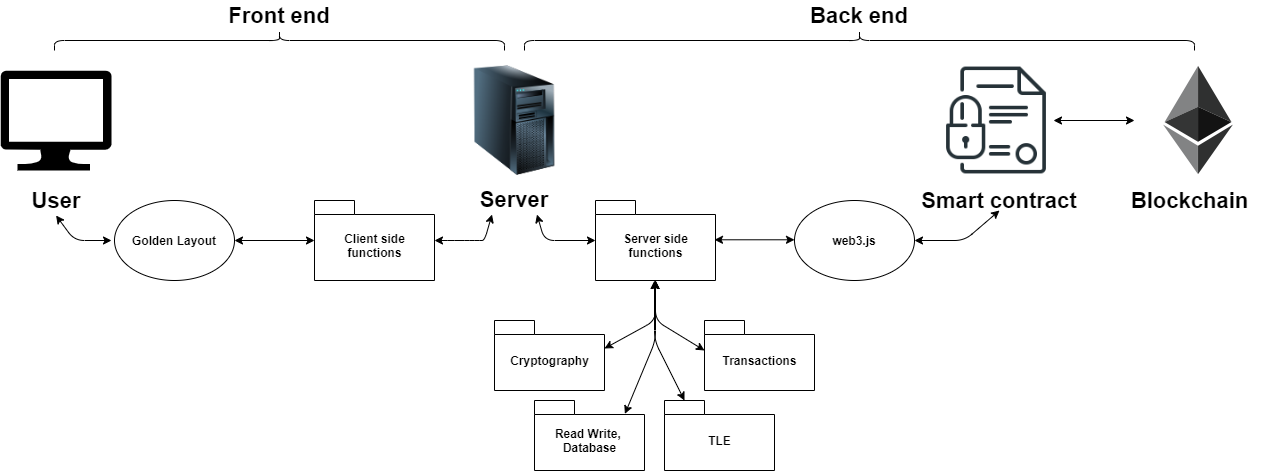
\includegraphics[width=\linewidth]{server.png}
 \caption{Architecture of the server}
 \label{fig:Front-end/back-end}
\end{figure*}


Let us take an example: suppose that Alice wants to send a new reference. Through the interface on her computer, she fills a form and writes the description of her reference, the initial price, the type of depreciation, how long the reference should last. When she clicks on the submit button, the browser validates the inputs or displays an error if it is necessary, and then sends a request to the server. The latter sends the information to the server-side functions, which form the transaction. The transaction is then sent to the blockchain, using web3.js. If everything goes well, web3.js returns a receipt, with amongst others the number of the block on which the transaction was registered, and the quantity of gas used. The server receives the receipt, and sends it to the client-side function that was waiting for a response. This function then displays the information to the user, for instance by changing a paragraph on the screen.

By separating front-end and back-end, we make sure we can change the interface without having to modify the interaction with the blockchain. In the same spirit, cryptography, transactions and handling the database are done in separate files. This disjunction also makes sure that our protocol does not depend on the server, as the goal of using a blockchain is to decentralize the process. Anyone could use the smart contracts, through another server.

\subsection{Cryptography}
If you wish to use the developped code from Github\cite{GitHub}, be aware that it is not perfectly secure. It was not designed to safely store keys. Our goal was simply to extensively test our smart contracts and prove the viability of our protocol. Be sure to only use it with test accounts. \textbf{Never use your personal key} before improving the security of the server. Our database is composed of .txt files containing the keys and messages, named after the client's/provider's address and the id of the object being sold. It is enough to test the protocol, but not secure enough to deploy in a real-life application.

All the cryptographic steps necessary off-blockchain were done in this server. We used \textit{Crypto}\cite{Crypto} which is a Node.js library for the Diffie-Hellman protocol and for generating random bytes. It is important to note that for the Diffie-Hellman exchange to function correctly, provider and client need to be using the same prime number and generators. Considering that these are not shared through the D-App, we fixed them in the server (see PrimeAndGenerator.txt). The prime number was generated once and stored in the database. We took a prime of length 1024 (we strongly recommend this being changed to 2048 bits). This length was not picked randomly: Odlyzko\cite{odlyzko} states that using a prime of at least 1024 bits is essential for moderate security, and 2048 bits for security valid over a decade. Finally, this prime generates keys which also are 1024 bits long, thus we slice them into 4 buffers of lengths 32 bytes to emit them through the contract, and concatenate these when they are received. The data to encrypt depends on the application. Since we are using an OTP, the key length will vary.
Initially the key was set as a \textit{bytes32} variable in the contract, but in this use case 49 bytes are necessary to encrypt the TLEs. Therefore we added a pseudo-random generator and the initial key $K$ became the seed for the real key. The seed length being of 32 bytes, no particular security threats arose.


\subsection{Designing the interface}
In order to have a user-friendly interface, we used Golden Layout\cite{GL}, created by Wolfram Hempel in 2014. This module allows to have native popout windows, and a responsive design. The point of using Golden Layout is that users can move the windows and stack them as they want. We made sure they couldn't open the same window twice.

With Golden Layout, the usual web pages are represented by components, which are displayed in their own window. It is these windows that Golden Layout allows to move and stack. Therefore, we listed the components to create, for example the list of connected nodes, the list of the most recent blocks or the list of bought items. After creating an empty layout, each of these components has to be registered in the layout. At this point the HTML content of the component is defined as the equivalent of the content of the web pages. Often, there are empty $<div>$ paragraphs identified with a unique id so that the content of this $<div>$ can be changed after executing a function.

When all the components are registered, it is time to initialise the layout. We can then choose which components will appear when the user opens the app: we decided to show the connection window and the list of blocks. This can easily be changed. The components that are not shown on the home page can be opened later on, as long as they have been registered. Some of them are accessible from the menu on the left part of the screen, and some of them open when clicking in a link in an already opened component.

\begin{figure*}[ht]
\centering
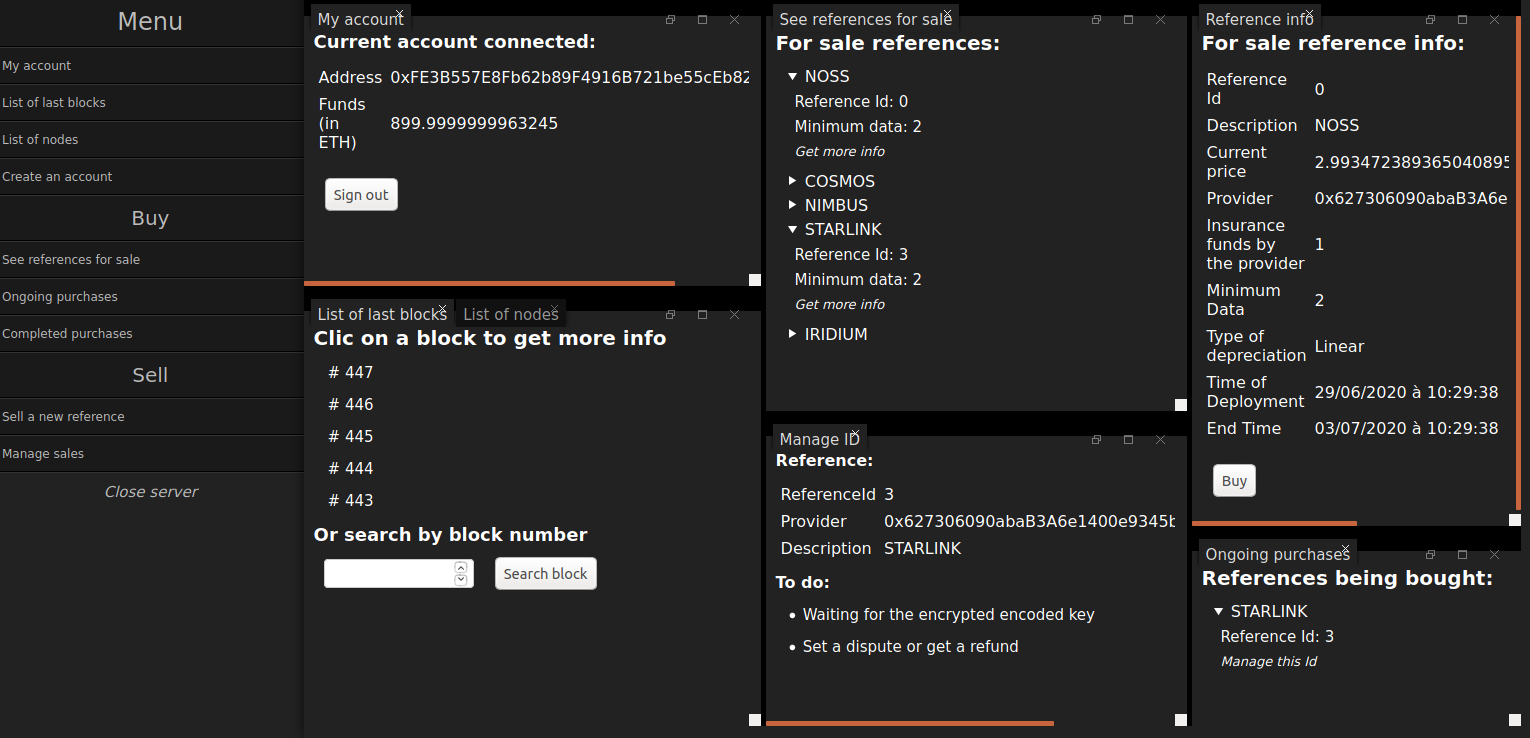
\includegraphics[width=\linewidth]{screenshot.png}
 \caption{A screenshot of the interface}
 \label{fig:Screenshot}
\end{figure*}

The menu helps to understand how the app is organized, as it is divided into three parts: the basic functionalities, the buyer part and the seller part.
\medskip
\subsubsection{Basic functionalities}
\paragraph{My account}
This component allows the users to connect to their account by entering their private key. They can then see the balance of their account, and their address is displayed. The connection allows the users to access specific parts of the app. For example one cannot buy a product without connecting beforehand. Theoretically the users can enter any private key, so they can access anyone's account. However as the private key is 256 bits long, the odds of guessing a randomly generated Ethereum private key is $1/2^{256}$. It is equivalent to finding a specific atom in the universe\cite{BlockchainBandit}.

\paragraph{List of last blocks}
This component displays the numbers of the latest blocks. The number of displayed blocks is a simple variable in the code and can be changed. By clicking on the number of a block, the users can see all of its details: the hash of both the block and the previous one, the miner, the timestamp... We also included an input field in the blocks list component, to get the info of any given block.

\paragraph{List of nodes}
Similarly to the block list, the users can see the list of nodes connected to the network. This is mainly for a debugging and pedagogical purpose.

\paragraph{Create an account}
When opening this component, the app creates an address and a private key with an empty balance. The users have the possibility to connect immediately with this newly created account. This functionality can be used to access the parts of the app that are blocked for a non connected user, for instance for demo purposes.
\medskip
\subsubsection{Buyer part}
\paragraph{See product for sale}
The content of this component is accessible to any user, connected or not. It displays all the items that are available for sale, using the HTML Details Element. When one clicks on the id of the product, the widget opens and a brief description is shown, as well as the price. Clicking on the ``Get more info'' link allows to see more info, such as the provider or the end time of the contract. If the users are connected, they can buy the product.

\paragraph{Ongoing purchases}
This component allows to see all the purchases that are not completed yet. As well as displaying the main info about the product, the app informs the user if there is a task to do, such as sending a hash if a provider answered the buy request. When the provider has sent $K_2$ the decoder key, the app allows the client to compute the reference key $K$ to access the data. There is also the possibility to set a dispute, or ask for a refund.

\paragraph{Completed purchases}
With this component, the users can access old purchases that are finished, so that they can see the TLEs in the reference. 

\medskip
\subsubsection{Seller part}
\paragraph{Sell a new product}
Once again, this component is accessible only to connected users. It consists in a form, to enter the basic information about the product the user is trying to sell. If the publication on the blockchain is successful, the user can see the number of the block on which was published the offer, the quantity of gas used and the reference ID given to the product.

\paragraph{Manage sales}
Similarly to the purchases component, the manage sales component allows to manage all the products that the user put on the market. There are several actions to do:
 \begin{itemize}
    \item Add a new TLE to the reference: fill in a form with the description of the space debris, and the two lines of the TLE;
    \item Send encrypted decoder keys $K \oplus K_2 \oplus K_3$ to clients (the app shows the number of clients waiting for that key);
    \item Verify received hashes and send $K_2$ to the correct clients;
    \item Release the reference key $K$ before the end of the contract;
    \item Withdraw money.
\end{itemize}

For testing purposes we coded \textit{malicious} versions of all functions which send a hash or a key. They represent ill-intended users and send random hashes or keys instead of correct ones.

\section{Benchmarks and Results}{\label{Benchmarks}}

As stated earlier, the server was modeled to test the logic of the functions and testify the viability of such a system. Since we could play the roles of different actors of the system (providers, clients, malicious entities) we were able to test all possible scenarios. These all proved to be correctly functional and gas usage was recorded.

The initial deployment of the smart contract costs 3 675 449 gas.

% gasUsed: 118583 with binary storage (with string object name not empty)
% gasUsed: 86650 with binary storage (and string object name is empty)

% gasUsed: 3530491, to deploy final version of the contract
% Previously: 4400000 gas used to deploy TLE
The only functions a client can call are detailed here with their gas costs. Keep in mind that a client only needs to call each function once. 
\begin{itemize}
    \item Buy function: varies between 126 000 and 128 000 gas depending on the parameters given by the provider.
    \item Send the hash: consistently costs 48 000 gas.
    \item Raise a dispute: this varies depending on the use case (simply a refund, or checking for a fraud), 27 600 gas was used in the worst case (need to compute a XOR and a hash).
\end{itemize}
This brings the client to a grand total of 181 600 gas (roughly \$1.02 at the time of writing) (refer to fig. \ref{fig:Client-Gas-Usage}). But keep in mind that most clients probably will not need to raise a dispute.

\begin{figure}[!htb]
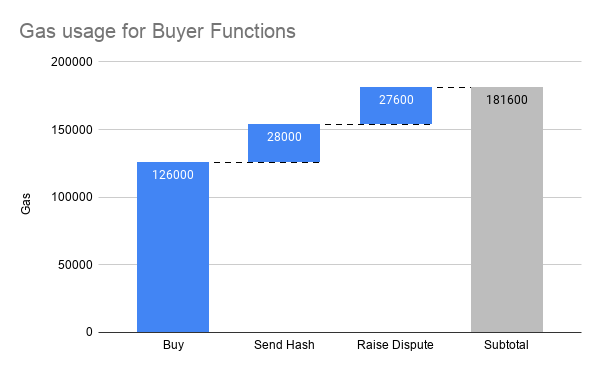
\includegraphics[width=\linewidth]{Gas usage for Buyer Functions.png}
 \caption{Client Gas Usage}
 \label{fig:Client-Gas-Usage}
\end{figure}


Concerning the provider, he must call several functions and some of which several times depending on what he intends to sell and to how many clients. Also sometimes the gas usage depends on the quantity of information he passes as parameters. Generally:
\begin{itemize}
    \item Selling a new reference : varies between 204 000 (no description) and 212 000 gas (100 characters used in the description).
    \item Send the encrypted decoder key ($K \oplus K_2 \oplus K_3$): consistently 28 400 gas (this function must be called for each client).
    \item Send decoder key $K_2$: 72 000 gas (also done for each client).
    \item Release the reference key $K$: consistently 45 600 gas. 
    \item Adding a new TLE to his reference: this greatly varies with the length of the Satellite Name (Line 0), from 86 850 gas if no characters are given, to 145 617 gas for a satellite name of 40 characters (although this is unthinkable). See fig. \ref{fig:TLE-Gas-Usage}.
    
\end{itemize}

    
\begin{figure}[!htb]
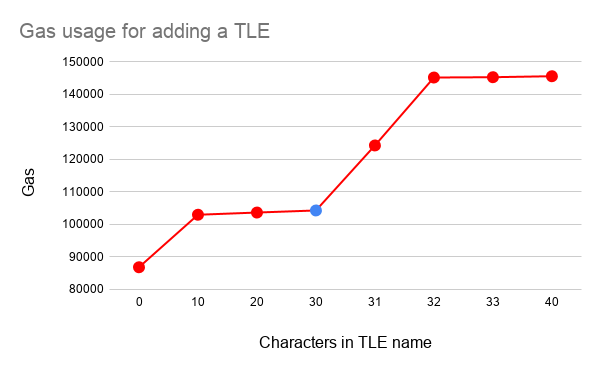
\includegraphics[width=\linewidth]{Gas usage for adding a TLE.png}
 \caption{Gas usage for adding a TLE}
 \label{fig:TLE-Gas-Usage}
\end{figure}

This brings the provider to a total of 453 000 gas (roughly \$2.53 at the time of writing). See fig. \ref{fig:Provider-Gas-Usage}.

\begin{figure}[!htb]
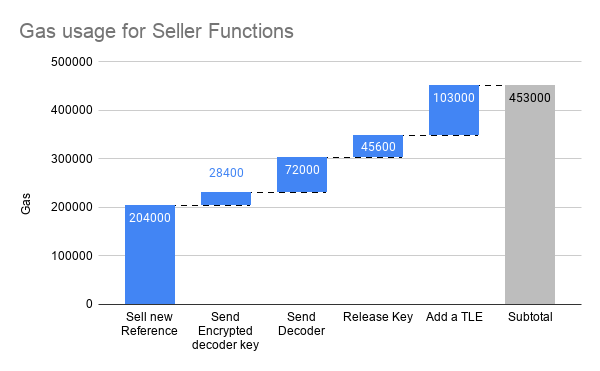
\includegraphics[width=\linewidth]{Gas usage for Seller Functions.png}
 \caption{Provider Gas usage}
 \label{fig:Provider-Gas-Usage}
\end{figure}

Since a provider probably won't sell only one TLE, a better example would be the expected cost for a full transaction of 10 TLEs and 50 clients. This would cost the provider roughly 6 299 600 gas  (\$ 40.19 today).

\section{Future work}{\label{Future work section}}

From what has been introduced in this paper, the smart contract is able to resolve disputes over the number of provided data and the correctness of the sent keys (fig. \ref{fig:Smart-Contract-Raise-Dispute}). However there are no guarantees that the provided data is correct or that the reference key indeed decrypts the data. For this situation, the reputation system that TruSat is developing would become handy, and even vital, to counterfeit this type of fraud. In future work it could be implicitly added that a provider could create a reference only if he meets a certain threshold of reputation. An ideal solution would be to evaluate the encrypted TLEs with TruSat's engine upon submission of the decryption key \textbf{K} at the end of the reference duration, and reward the reference's owner with the respective reputation points. If the redeemed points were not enough, the clients could reclaim their funds.  The smart contract could finally guarantee to both the client and the provider all their rights without the need of a centralized and trusted third party,.

Moreover, elaborating a secure client interface to communicate with this smart contract must be achieved if we hope to use it securely: a simple idea could be asking users to write them down and insert them when needed instead of storing the generated keys.

Finally, a formal proof over the security of the smart contract should be extensively studied before deployment.


\section{Conclusion}
The use of the developed protocol best fits fast depreciable information so that revealing the reference decryption key after a few days will not affect the seller or the buyer. In addition a reputation system like the one proposed by TruSat is strongly recommended to evaluate the encrypted data without a third party and ensure they withhold real value. Nevertheless the smart contract can be used outside the scope of space debris: with minor changes it can befit meteorological data. Even yet one could create a platform to exchange trading signals, which would be relatively easy and practical. 

The main issue however comes from the gas consumption and price as well as the possible flood of transactions needed on the blockchain for an application such as TruSat. If 100 000 space objects are reported daily, which is highly achievable, it would raise the total amount of transactions per day by 10\% validated on the Ethereum mainnet. A similar scenario occured after the launch of ``CryptoKitties", a D-App to raise virtual kitties, which caused a huge congestion in the network and a spike of the gas price \cite{Kitties}.

In the future, with the launch of the Proof of Stake consensus mechanism, more transactions could be processed on the Ethereum mainnet and hopefully the limitation on gas price and usage won't hinder deploying TruSat as well as the Depreciation Contract to ensure a safer space.

One of the biggest advantages of using a Public Ledger is not only promoting the collaboration between existing agencies, but also assisting in the creation of small startups in the space sector. With a simple contract, small scale companies could join forces and share their information in order to sell their services or data to other parties. With a constellation of CubeSats integrated with a passive bistatic radar \cite{CubesatPBR}, tracking could be done at affordable costs. As stated in ``Blockchain application within a multi-sensor satellite architecture'' \cite{BlockchainMultiSensor}, the distribution of tasks and the automation of observation would be possible.

Collision assessment businesses such as \href{https://www.agi.com/home}{\textit{AGI company}} do not only sell services for tracking space objects but also developing algorithms and tools to process all of the data collected and predict collisions as well as compute the probability of such collisions. According to a 2012 international conference, after applying clustering techniques it costs 2 hours of computing power to analyse collision risks with a sample of 15 000 objects when using a computer of eight blades and 128 cores within 32 processors \cite{ParallelComputing}.

 The immutable specificity of blockchains comes in handy for researchers as they can use the blockchain's database to develop their algorithms and hence improve private companies' collision assessment predictions and efficiency. When adding 300 000 objects to the tracking list, computing requirements become more hefty and specialised algorithms or services tend to be more appealing.
%% TODO

% To store string TLE without any compression:
% 168468 gas if we delete spaces versus
% 190720 gas if we do not delete spaces
% FINAL VERSION GASSES:

% Sell new reference with no description: 204000 (consistent)
% Sell new reference with 100 character description: 212000 (consistent) (10 charac = 800 gas ella awal 10 b shi 950 bas ensa)

% Upload TLE with no satellite name: 86850 gas
% Upload TLE with 10 character satellite name: 103000
% Upload TLE with 20 character satellite name: 103680
% Upload TLE with 30 character satellite name: 104320
% Upload TLE with 31 character satellite name: 124320
% Upload TLE with 32 character satellite name: 145217
% Upload TLE with 33 character satellite name: 145217+chi
% Upload TLE with 40 character satellite name: 145617





% Buy function 126 000 (marten ejet) - 128 000 gas

% Send k xor k2 xor xor k3: 28400 gas (marten ejet)

% Send hash 48 000 gas (marten ejet)

% Send decoder k2: 72000 gas (marten ejet)

% Release Key: 45600 gas (marra)

% Max raise dispute: 27600 gas (case when release key is not correct yaane 3melna keccack w xor arranehon w ba3atna funds lal client)




% Typical expected cost for a full transaction of: 10TLE's and 50 clients:
% Clients will pay: 181600 gas (1.15861 dollars today)
% In total, the provider will pay: 
% -6299600 gas  (40.19145 dollars today)

% Graph showing for the provider at what time the clients bought and at which price 
\bibliographystyle{plain}
\bibliography{references}


\end{document}